\documentclass[11pt]{article}
\usepackage[margin=1in]{geometry}
\usepackage[T1]{fontenc}
\usepackage[utf8]{inputenc}
\usepackage{lmodern}
\usepackage{microtype}
\usepackage{amsmath,amssymb}
\usepackage{booktabs}
\usepackage{siunitx}
\usepackage{graphicx}
\usepackage{xcolor}
\usepackage{array}
\usepackage{hyperref}
\usepackage{pgfplots}
\pgfplotsset{compat=1.18}
\sisetup{round-mode=places, round-precision=3}
\hypersetup{colorlinks=true, linkcolor=blue!50!black,
            citecolor=blue!50!black, urlcolor=blue!50!black}

\title{%
  ClassicObby-RL: Training a Deep Q-Network Agent \\
  to Navigate a Roblox Obstacle Course
}
\author{Nathan L.}
\date{April 18, 2026}

\begin{document}
\maketitle

% ---------------------------------------------------------------
\begin{abstract}
ClassicObby-RL is an end-to-end reinforcement learning system that trains
a Deep Q-Network agent to autonomously navigate a Roblox Classic Obstacle
Course (obby). The agent observes a 25-dimensional state vector encoding
kinematics, spatial rays, edge probes, and hazard proximity, and selects
from seven discrete movement actions. A Python Flask training server
communicates with the Roblox game engine in real time via HTTP, performing
online policy updates with a dueling network architecture, NoisyLinear
exploration, prioritised experience replay, and $n$-step returns. Over a
recorded window of 10{,}759 steps spanning 498 completed episodes, the
mean terminal episode return rises from 1.29 in the first fifth of
training to 18.79 in the final fifth---an improvement of 17.49 points---
while median serving latency remains below \SI{41}{ms}. This report
presents the full system design, learning algorithm, and a quantitative
analysis of the training results.
\end{abstract}

% ---------------------------------------------------------------
\section{Introduction}
\label{sec:intro}

Roblox obstacle courses, known colloquially as \emph{obbies}, challenge a
player character to jump across platforms, avoid lethal hazards, and pass
through a sequence of checkpoints inside a three-dimensional game world.
The task requires precise timing, spatial awareness, and adaptive recovery
from failures, making it a natural testbed for discrete-action
reinforcement learning: the state space is continuous and
high-dimensional, rewards are sparse at checkpoint boundaries, and each
episode ends either in failure (a fall or hazard collision) or in success
(reaching the final checkpoint).

ClassicObby-RL implements the learning loop \emph{online}, meaning the
agent generates experience by controlling a live Roblox character while
simultaneously updating its policy. This design creates a tight coupling
between the Roblox engine, an HTTP communication layer, and the PyTorch
training code. The primary engineering challenge is keeping per-step
inference and training latency low enough that the agent can make
decisions at a useful rate without interrupting the game's physics
simulation.

This report is structured as follows. Section~\ref{sec:arch} describes
the system architecture and inter-component data flow. Section~\ref{sec:agent}
defines the observation space, action space, and reward function.
Section~\ref{sec:algo} presents the learning algorithm and its
enhancements. Section~\ref{sec:results} reports quantitative training
results with supporting figures. Section~\ref{sec:discussion} discusses
strengths and limitations, and Section~\ref{sec:conclusion} concludes.

% ---------------------------------------------------------------
\section{System Architecture}
\label{sec:arch}

The system is composed of three loosely coupled components that
communicate via Roblox's internal RemoteFunction mechanism and HTTP.

\paragraph{Roblox client (\texttt{AgentClient.client.lua}).}
A LocalScript running inside the Roblox client collects observations from
the character's \texttt{HumanoidRootPart}, computes auxiliary shaping
terms locally, and packages everything into a JSON payload. It invokes
the \texttt{RLStep} RemoteFunction at a configurable decision interval
(0.25\,s by default), receives an action integer in response, and applies
the corresponding movement command to the character. The client also
maintains bookkeeping for checkpoint tracking, stuck detection, hazard
proximity, and episode boundary detection.

\paragraph{Roblox server bridge (\texttt{RLServer.lua}).}
A ServerScript listens on the \texttt{RLStep} RemoteFunction. On each
invocation it serialises the client payload and forwards it to the Python
server's \texttt{/step} endpoint via \texttt{HttpService:PostAsync}.
It then decodes the JSON response and returns the selected action integer
to the client. This thin bridge isolates the Python training code from
Roblox's networking constraints and allows the server to be restarted
without affecting the in-progress game session.

\paragraph{Python training server (\texttt{rl\_server.py}).}
A Flask application exposes a \texttt{/step} POST endpoint. On each
request it normalises the incoming observation, selects an action using
the Q-network, stores the transition in a prioritised replay buffer, and
performs a gradient update every \texttt{update\_every} steps. The best
checkpoint by episode return is saved to \texttt{checkpoints/best.pt},
and all per-step data---step count, episode number, action, reward,
serving latency, exploration rate, and Q-loss---are appended to
\texttt{training\_metrics.csv}. A separate \texttt{config\_manager.py}
module loads all tuneable parameters at startup from two configuration
files:
\begin{itemize}
  \item \texttt{config/model\_config.yaml} -- network architecture and
    training hyperparameters;
  \item \texttt{config/reward\_shaping.conf} -- all reward magnitudes and
    detection thresholds.
\end{itemize}
Both files can be edited and hot-reloaded at runtime, allowing reward and
architecture experiments without a server restart.

The data flow between the three components is summarised below:

\begin{center}
\renewcommand{\arraystretch}{1.3}
\small
\begin{tabular}{@{}c@{\quad$\longrightarrow$\quad}c@{\quad$\longrightarrow$\quad}c@{}}
  \textbf{Roblox client} & \textbf{Roblox server bridge} &
  \textbf{Python training server} \\
  observation, shaped reward & HTTP POST \texttt{/step} & action integer \\
\end{tabular}
\end{center}

% ---------------------------------------------------------------
\section{Agent Design}
\label{sec:agent}

\subsection{Observation Space}

The agent receives a 25-dimensional observation vector $s_t \in
\mathbb{R}^{25}$ at each decision step. The features are divided into
four semantic groups.

\begin{enumerate}
  \item \textbf{Goal-relative kinematics} (\texttt{dx}, \texttt{dy},
    \texttt{dz}, \texttt{vx}, \texttt{vy}, \texttt{vz}): the signed
    displacement and velocity of the character root relative to the next
    checkpoint position. These six features give the agent a
    goal-directed sense of direction and momentum at all times.

  \item \textbf{Ground contact and locomotion state} (\texttt{down},
    \texttt{forward}, \texttt{angle}, \texttt{grounded}, \texttt{speed},
    \texttt{tJump}): the distance to the ground below and to any obstacle
    directly ahead (both via raycasting), the cosine of the angle between
    the character's look direction and the goal direction, a binary
    grounded flag, horizontal speed, and the time elapsed since the last
    jump (capped at 5\,s for normalisation).

  \item \textbf{Radial obstacle rays} (\texttt{r0}--\texttt{r7}): eight
    equally spaced horizontal raycasts emanating from the character at
    ground level, covering all 360 degrees in 45-degree increments. Together
    they encode the surrounding obstacle geometry, allowing the agent to
    detect walls and platform edges without requiring a full 3-D scene
    representation.

  \item \textbf{Hazard and edge probes} (\texttt{dropF}, \texttt{dropR},
    \texttt{dropL}, \texttt{hazardDist}, \texttt{lastDeathType}): three
    downward raycasts projected a short distance ahead, to the right, and
    to the left of the character to detect upcoming ledge drops; the
    normalised distance to the nearest hazard-tagged object; and an
    integer encoding the type of the most recent death event (0 = none,
    1 = hazard, 2 = fall, 3 = other).
\end{enumerate}

All observations are standardised online using a running mean and
variance estimator (\texttt{RunningNorm}). Normalisation is disabled for
the first 100 steps so that the running statistics can warm up before
being applied.

\subsection{Action Space}

The agent selects one of seven discrete actions at each decision step,
as listed in Table~\ref{tab:actions}. Actions are applied at the
character level for the full duration of the 0.25\,s decision window.
Action~5 applies an additional linear impulse boost in the forward
direction during the jump to enable the agent to clear longer platform
gaps.

\begin{table}[htbp]
  \centering
  \caption{Discrete action set available to the agent at each step.}
  \label{tab:actions}
  \begin{tabular}{cll}
    \toprule
    ID & Action & Description \\
    \midrule
    0 & Idle             & No movement input; the character decelerates naturally \\
    1 & Forward          & Move in the character's current look direction \\
    2 & Strafe left      & Move perpendicular-left relative to the look direction \\
    3 & Strafe right     & Move perpendicular-right relative to the look direction \\
    4 & Jump             & Jump vertically in place \\
    5 & Forward + Jump   & Move forward and jump; a horizontal impulse boost is applied \\
    6 & Backward         & Move opposite to the current look direction \\
    \bottomrule
  \end{tabular}
\end{table}

\subsection{Reward Shaping}

Because checkpoint rewards are sparse, a dense reward shaping scheme
provides continuous feedback throughout each episode. The shaping
signal is computed entirely on the Roblox client and transmitted to
the server as part of each step payload, ensuring the logged reward
values are ground-truth measurements from the game engine.
Table~\ref{tab:rewards} summarises every reward component and its
configured magnitude.

\begin{table}[htbp]
  \centering
  \caption{Reward shaping components as configured in
    \texttt{reward\_shaping.conf}.}
  \label{tab:rewards}
  \begin{tabular}{lrp{6.5cm}}
    \toprule
    Component & Magnitude & Trigger condition \\
    \midrule
    Progress reward  & $5.0 \times \Delta d$   &
      Per step; proportional to improvement in distance to the next
      checkpoint. Negative when the agent moves away, capped at
      $-1.0$. \\
    Leap bonus       & $+2.0$    &
      A single step in which the agent moves ${\geq}1.5$\,studs
      closer to the goal. \\
    Milestone bonus  & $+5.0$    &
      Every $0.5$-stud improvement beyond the agent's best-ever
      distance to the current checkpoint. \\
    Sustained bonus  & $+1.0$    &
      Each step with consistent progress exceeding $0.3$\,studs. \\
    Checkpoint bonus & $+50.0$   &
      Reaching the next numbered checkpoint. \\
    Completion bonus & $+100 + 20n$ &
      Finishing all checkpoints; $n$ is the total checkpoint count. \\
    Base step cost   & $-0.001$  &
      Applied every step to discourage indefinite idling. \\
    Hazard death     & $-5.0$    &
      Dying by contact with a \texttt{CollectionService}-tagged
      hazard part. \\
    Fall death       & $-3.0$    &
      Dying by falling below the map's fall boundary. \\
    Stuck penalty    & $-3.0$    &
      No measurable progress for 200 consecutive steps. \\
    \bottomrule
  \end{tabular}
\end{table}

The combination of dense progress shaping with sparse checkpoint bonuses
guides the agent toward continuous forward motion while explicitly
discouraging hazard contact and prolonged stagnation. Because all
magnitudes are loaded from a configuration file at startup, reward
experiments can be conducted without modifying or restarting the server.

% ---------------------------------------------------------------
\section{Learning Algorithm}
\label{sec:algo}

\subsection{Dueling Network Architecture}

The Q-network uses a dueling architecture~\cite{wang2016} that separates
state-value estimation from action-advantage estimation. A shared feature
extractor---two fully connected layers of width 512, each followed by
Layer Normalisation and a ReLU activation---maps the normalised
observation to a latent representation. Two independent heads, each with
one hidden layer of width 256, then compute the value stream $V_\theta(s)$
and advantage stream $A_\theta(s, a)$. The Q-values are recovered via

\begin{equation}
  Q_\theta(s,a) = V_\theta(s) + A_\theta(s,a) -
  \frac{1}{|\mathcal{A}|}\sum_{a'} A_\theta(s,a'),
  \label{eq:dueling}
\end{equation}

where subtracting the mean advantage improves identifiability of the
value and advantage functions~\cite{wang2016}. When
\texttt{use\_noisy\_nets} is enabled, the linear layers in both heads
are replaced with NoisyLinear layers~\cite{fortunato2018}, which add
learned factorised Gaussian noise to weights and biases. This provides
state-dependent intrinsic exploration without relying solely on the
outer $\varepsilon$-greedy schedule.

\subsection{Training Enhancements}

The training loop extends vanilla DQN~\cite{mnih2015} with four
additional mechanisms.

\begin{itemize}
  \item \textbf{Prioritised Experience Replay (PER)~\cite{schaul2016}.}
    Transitions are stored in a sum-tree buffer and sampled
    proportionally to their TD-error raised to priority exponent
    $\alpha = 0.7$. Importance-sampling weights with $\beta$ annealed
    from 0.4 toward 1.0 correct the resulting distributional bias.

  \item \textbf{$n$-step returns.} Rather than a one-step Bellman
    target, the agent bootstraps from a 5-step return,
    $y_t = \sum_{k=0}^{4} \gamma^k r_{t+k} + \gamma^5
    \max_{a'} Q_{\theta^-}(s_{t+5}, a')$, which reduces variance in
    the value estimate and accelerates credit assignment across
    multi-platform sequences.

  \item \textbf{Soft target network updates.} The target network
    $\theta^-$ is updated after every optimisation step via a Polyak
    average, $\theta^- \leftarrow (1-\tau)\,\theta^- + \tau\,\theta$,
    with $\tau = 0.02$. This provides a more stable regression target
    than periodic hard copies while still tracking the online network
    closely.

  \item \textbf{Online observation normalisation.} A running
    mean-and-variance estimator standardises each observation before it
    enters the network. The normalisation state is saved inside
    checkpoints so that it is preserved across restarts.
\end{itemize}

The loss is the importance-weighted Huber (SmoothL1) loss,

\begin{equation}
  \mathcal{L}(\theta) =
  \mathbb{E}_{(s,a,r,s') \sim \mathcal{B}}
  \!\left[\,w_i \cdot \ell_\delta\!\left(Q_\theta(s,a) - y_i\right)\right],
  \label{eq:loss}
\end{equation}

where $y_i$ is the $n$-step target and $w_i$ are the PER
importance-sampling weights. Gradient norms are clipped to 2.0 to
prevent destabilising updates early in training.

\subsection{Hyperparameters}

Table~\ref{tab:hyper} lists all model and training hyperparameters used
during the logged training run.

\begin{table}[htbp]
  \centering
  \caption{Model and training hyperparameters used throughout the
    logged run.}
  \label{tab:hyper}
  \begin{tabular}{lrl}
    \toprule
    Parameter & Value & Notes \\
    \midrule
    \multicolumn{3}{l}{\textit{Network}} \\
    Shared hidden width   & 512     & Two-layer feature extractor \\
    Value / adv.\ hidden  & 256     & Per-stream hidden layer \\
    Noise $\sigma_\text{init}$ & 0.5 & NoisyLinear initial noise scale \\[2pt]
    \multicolumn{3}{l}{\textit{Optimisation}} \\
    Optimiser             & AdamW   & Weight decay $= 10^{-5}$ \\
    Learning rate         & $10^{-3}$ & Fixed throughout \\
    Discount $\gamma$     & 0.98    & \\
    $n$-step horizon      & 5       & \\
    Batch size            & 128     & \\
    Update frequency      & 1       & Gradient step every environment step \\
    Gradient clip         & 2.0     & Max gradient norm \\[2pt]
    \multicolumn{3}{l}{\textit{Exploration}} \\
    $\varepsilon_\text{start}$ & 0.30 & Initial epsilon \\
    $\varepsilon_\text{min}$   & 0.01 & Minimum epsilon \\
    $\varepsilon_\text{decay}$ & 0.99 & Per-step multiplicative decay \\[2pt]
    \multicolumn{3}{l}{\textit{Replay buffer}} \\
    Buffer capacity       & 50{,}000 & \\
    PER $\alpha$          & 0.70    & Priority exponent \\
    PER $\beta_\text{start}$ & 0.40 & IS-weight annealing start \\
    Target update $\tau$  & 0.02    & Soft Polyak coefficient \\
    \bottomrule
  \end{tabular}
\end{table}

% ---------------------------------------------------------------
\section{Results}
\label{sec:results}

All results are derived from \texttt{training\_metrics.csv}, which was
produced by a continuous online training session. The log begins at
environment step 2{,}457 with $\varepsilon = 0.01$, indicating that the
exploration phase had already concluded before this window was recorded.
The agent is therefore operating almost entirely in exploitation mode,
with residual NoisyNet-driven stochastic exploration.

\subsection{Training Progress}

Figure~\ref{fig:reward_step} shows both the per-step reward and the
cumulative within-episode reward over all 10{,}759 logged steps. The
cumulative trace resets to zero at the start of each new episode, so
ascending arcs correspond to uninterrupted forward progress through the
level, while sharp drops indicate deaths or forced resets. In the first
half of the log, short episodes with mostly negative or near-zero
terminal returns dominate. In the second half, longer ascending arcs
appear with increasing frequency, reflecting the policy's growing ability
to chain together successful platform crossings.

\begin{figure}[htbp]
  \centering
  \begin{tikzpicture}
    \begin{axis}[
      width  = 0.95\linewidth,
      height = 0.36\textheight,
      xlabel = {Environment step},
      ylabel = {Reward},
      title  = {Per-Step and Cumulative Episode Reward vs.\ Step},
      legend pos  = north west,
      grid        = both,
      grid style  = {line width=0.3pt, gray!35},
      line width  = 0.7pt,
      xmin = 2457, xmax = 13215,
    ]
      \addplot[color=blue!60!black, opacity=0.50, line width=0.6pt]
        table[x=step_count, y=reward,
              col sep=comma, each nth point=12]
        {training_metrics.csv};
      \addlegendentry{Per-step reward}
      \addplot[color=red!70!black, opacity=0.90, line width=1.2pt]
        table[x=step_count, y=episode_reward,
              col sep=comma, each nth point=12]
        {training_metrics.csv};
      \addlegendentry{Cumulative episode reward}
    \end{axis}
  \end{tikzpicture}
  \caption{Per-step reward (blue, faint) and cumulative within-episode
    reward (red, bold) across the full logged training window. Drops to
    negative values in the cumulative trace mark deaths; subsequent
    ascents reflect the policy successfully accumulating positive
    progress rewards. Both signals trend upward in the second half of
    the window, consistent with the quantitative improvement documented
    in Table~\ref{tab:trend}.}
  \label{fig:reward_step}
\end{figure}

\subsection{Episode-Level Statistics}

Table~\ref{tab:core} summarises aggregate statistics computed from all
logged steps. Table~\ref{tab:trend} compares episode returns at the
beginning and end of the training window to quantify the degree of
improvement over time.

\begin{table}[htbp]
  \centering
  \caption{Aggregate training and serving statistics across all
    10{,}759 logged steps.}
  \label{tab:core}
  \begin{tabular}{lr}
    \toprule
    Metric & Value \\
    \midrule
    Total logged steps                    & 10{,}759 \\
    Unique episodes                       & 499 \\
    Completed episodes (\texttt{done=True}) & 498 \\
    Mean per-step reward                  & 0.477 \\
    Per-step reward standard deviation    & 3.880 \\
    Mean cumulative episode reward        & 10.774 \\
    Maximum cumulative episode reward     & 117.222 \\
    Minimum cumulative episode reward     & $-$68.049 \\
    Mean HTTP request latency             & \SI{40.89}{ms} \\
    Median HTTP request latency           & \SI{40.27}{ms} \\
    95th-percentile HTTP latency          & \SI{64.66}{ms} \\
    Maximum HTTP request latency          & \SI{104.08}{ms} \\
    Steps with non-zero Q-loss            & 10{,}494 \\
    \bottomrule
  \end{tabular}
\end{table}

\begin{table}[htbp]
  \centering
  \caption{Episode-level trend: mean terminal return in the first and
    last 20\% of the 498 completed episodes.}
  \label{tab:trend}
  \begin{tabular}{lr}
    \toprule
    Metric & Value \\
    \midrule
    Completed episodes analysed              & 498 \\
    First 20\% mean terminal return          & 1.29 \\
    Last 20\% mean terminal return           & 18.79 \\
    Absolute improvement                     & $+$17.49 \\
    Episodes with a positive terminal return & 68.1\% \\
    Best single-episode return (ep.\ 215)    & 95.77 \\
    Worst single-episode return (ep.\ 449)   & $-$63.93 \\
    \bottomrule
  \end{tabular}
\end{table}

The 14.5$\times$ improvement in mean terminal return between the first
and last quintiles confirms that the policy is learning, not merely
oscillating around a fixed baseline. The high per-step reward standard
deviation (3.88) reflects the bimodal step-reward distribution:
most steps yield either a scaled progress reward or a death penalty of
$-5.0$, with shaped intermediate values occurring less frequently.
The 68.1\% positive-terminal-return rate further indicates that the
policy ends the majority of episodes having accumulated net positive
shaped reward, even though explicit checkpoint completions require
traversing the full course.

\subsection{Policy Behaviour: Action Distribution}

Figure~\ref{fig:actions} shows the total number of times each of the
seven actions was selected across all 10{,}759 logged steps.

\begin{figure}[htbp]
  \centering
  \begin{tikzpicture}
    \begin{axis}[
      ybar,
      width  = 0.90\linewidth,
      height = 0.30\textheight,
      xlabel = {Action},
      ylabel = {Selection count},
      title  = {Action Selection Frequency Across All Logged Steps},
      xtick  = data,
      xticklabels = {%
        0\ (Idle), 1\ (Fwd), 2\ (Left), 3\ (Right),
        4\ (Jump), 5\ (Fwd+Jump), 6\ (Back)},
      x tick label style = {rotate=30, anchor=east, font=\small},
      nodes near coords,
      nodes near coords align = {vertical},
      nodes near coords style = {font=\small},
      bar width  = 18pt,
      ymin       = 0,
      grid       = major,
      grid style = {gray!30},
      enlarge x limits = 0.08,
    ]
      \addplot[fill=orange!70!yellow, draw=orange!60!black] coordinates {
        (0,3426)
        (1,2602)
        (2,2212)
        (3,1685)
        (4,4)
        (5,696)
        (6,134)
      };
    \end{axis}
  \end{tikzpicture}
  \caption{Frequency of each action across 10{,}759 logged steps. The
    policy strongly favours idle and directional movement over
    jump-based actions, with action~4 (jump in place) selected only
    four times.}
  \label{fig:actions}
\end{figure}

The policy overwhelmingly favours actions 0--3, which involve
horizontal movement or idling without jumping. Action~5 (forward jump)
accounts for 696 of the 10{,}759 decisions---the only jump variant
used with meaningful frequency. This preference is rational given the
reward structure: the progress reward scales with horizontal distance
improvement, so combining forward movement and jumping in a single action
(action~5) yields more reward per step than a jump in place (action~4)
followed by a separate forward step. Action~6 (backward) appears just
134 times, suggesting the agent employs it sparingly for positional
corrections rather than as a primary navigation strategy. Action~4's
near-absence (4 selections) indicates the policy has effectively learned
that isolated vertical jumps do not contribute to progress in this map
layout.

\subsection{Serving Latency}

Figure~\ref{fig:latency} shows the HTTP round-trip latency for each
decision step over the full training window.

\begin{figure}[htbp]
  \centering
  \begin{tikzpicture}
    \begin{axis}[
      width      = 0.95\linewidth,
      height     = 0.30\textheight,
      xlabel     = {Environment step},
      ylabel     = {Latency (ms)},
      title      = {HTTP Round-Trip Latency per Decision Step},
      grid       = both,
      grid style = {line width=0.3pt, gray!35},
      ymin = 0, ymax = 115,
      xmin = 2457, xmax = 13215,
      line width = 0.7pt,
      color      = teal!70!black,
    ]
      \addplot
        table[x=step_count, y=request_time_ms,
              col sep=comma, each nth point=12]
        {training_metrics.csv};
      \draw[dashed, red!65!black, line width=0.9pt]
        (axis cs:2457,64.66) -- (axis cs:13215,64.66)
        node[pos=0.96, above, font=\small] {P95 (\SI{64.66}{ms})};
    \end{axis}
  \end{tikzpicture}
  \caption{Per-step HTTP round-trip latency between the Roblox bridge
    and the Python training server. The dashed line marks the 95th
    percentile. The vast majority of requests complete in under
    \SI{50}{ms}; occasional spikes above this level are consistent with
    OS scheduling jitter or Python garbage collection pauses.}
  \label{fig:latency}
\end{figure}

With a median of \SI{40.27}{ms} and a P95 of \SI{64.66}{ms}, the server
handles every decision request well within the 250\,ms decision window.
The maximum observed latency of \SI{104.08}{ms} is less than half of
that budget, so even worst-case delays do not cause decision steps to be
dropped. These figures also confirm that the combined cost of observation
normalisation, forward pass, PER sampling, and a gradient update fits
comfortably in the available per-step time on a standard CPU.

% ---------------------------------------------------------------
\section{Discussion}
\label{sec:discussion}

\paragraph{Strengths.}
The system demonstrates that end-to-end online RL is practical in a live
game engine with strict latency constraints. The fully modular configuration
system makes reward shaping and architecture iteration straightforward:
changing a reward magnitude requires editing a single \texttt{.conf} file,
and the change takes effect on the next server reload without interrupting
an ongoing training session. Checkpointing preserves the best policy and
observation-normalisation statistics across restarts, and the
\texttt{train\_offline.py} utility allows rapid hyperparameter search in a
synthetic environment without requiring a running Roblox session.

\paragraph{Limitations.}
The results come from a single continuous log rather than multiple
independent seeds, so the observed improvement cannot be attributed to
policy learning with statistical confidence. The log also begins at step
2{,}457 with $\varepsilon$ already at its minimum value, indicating that
earlier exploration and warm-up phases are not captured here. The CSV
schema does not include an explicit course-completion flag, making it
impossible to compute a success rate directly; completion can only be
inferred from unusually high episode returns. Finally, the near-complete
absence of action~4 (jump in place) suggests the policy may have
converged to a locally optimal movement strategy that avoids obstacles
requiring precise vertical jumps without forward momentum, pointing to a
potential performance ceiling that multi-seed experiments and reward
ablations could clarify.

\paragraph{Future directions.}
Promising next steps include conducting multi-seed evaluations with fixed
initialisations, adding an explicit course-completion flag to the step
log, implementing curriculum learning by progressively unlocking
checkpoints, and comparing the current DQN variant against
continuous-control algorithms such as PPO or SAC adapted to the discrete
action space.

% ---------------------------------------------------------------
\section{Conclusion}
\label{sec:conclusion}

ClassicObby-RL is a complete, working reinforcement learning system for
navigating a Roblox obstacle course in real time. It demonstrates that a
dueling DQN agent augmented with NoisyLinear exploration, prioritised
experience replay, and $n$-step returns can learn meaningful locomotion
policies inside a live game engine using a standard CPU and a local HTTP
connection. The recorded training window shows a clear improvement in
terminal episode returns---from a mean of 1.29 in the earliest episodes
to 18.79 in the latest---alongside stable sub-\SI{41}{ms} median serving
latency throughout. The fully configurable codebase, offline training
support, and runtime parameter reloading make the project a practical
foundation for further reinforcement learning research in interactive
three-dimensional environments.

% ---------------------------------------------------------------
\begin{thebibliography}{9}

\bibitem{mnih2015}
V.~Mnih, K.~Kavukcuoglu, D.~Silver, et al.,
``Human-level control through deep reinforcement learning,''
\emph{Nature}, vol.~518, no.~7540, pp.~529--533, 2015.

\bibitem{wang2016}
Z.~Wang, T.~Schaul, M.~Hessel, H.~van Hasselt, M.~Lanctot, and N.~de
Freitas,
``Dueling network architectures for deep reinforcement learning,''
in \emph{Proc.\ International Conference on Machine Learning (ICML)},
2016.

\bibitem{fortunato2018}
M.~Fortunato, M.~G.~Azar, B.~Piot, et al.,
``Noisy networks for exploration,''
in \emph{Proc.\ International Conference on Learning Representations
(ICLR)}, 2018.

\bibitem{schaul2016}
T.~Schaul, J.~Quan, I.~Antonoglou, and D.~Silver,
``Prioritized experience replay,''
in \emph{Proc.\ International Conference on Learning Representations
(ICLR)}, 2016.

\bibitem{sutton2018}
R.~S.~Sutton and A.~G.~Barto,
\emph{Reinforcement Learning: An Introduction}, 2nd~ed.
MIT Press, Cambridge, MA, 2018.

\end{thebibliography}

\end{document}
